%!TEX program = lualatex

\documentclass{sintefbeamer}
\usepackage{amsfonts,amsmath,oldgerm}

\usepackage{unicode-math}

\usepackage{tikz}
\usetikzlibrary{positioning,shapes,arrows,calc,intersections}
\usepackage{pgfplots}
\pgfplotsset{compat=1.8}

\definecolor{darkblue}{HTML}{00688B}
\definecolor{darkgreen}{HTML}{6E8B3D}
\definecolor{mediumgreen}{HTML}{008000}
\definecolor{cadet}{HTML}{DAE1FF}
\definecolor{salmon}{HTML}{FFB08A}

\newcommand{\testcolor}[1]{\colorbox{#1}{\textcolor{#1}{test}} \texttt{#1}}

\usefonttheme[onlymath]{serif}

\newcommand{\hrefcol}[2]{\textcolor{cyan}{\href{#1}{#2}}}

\title{Interpolated models for non-intrusive affinization of reduced basis methods}
\author{\href{mailto:eivind.fonn@sintef.no}{Eivind Fonn}, Harald van Brummelen, Jens Eftang, Trond Kvamsdal, Adil Rasheed}
\date{June 9, 2022}

\begin{document}

\maketitle

\begin{frame}{Contents}
    \begin{itemize}
        \item The what: jacket joint components
        \item The plan (part 1): port condensation ROM technique
        \item The plan (part 2): thoughts about intrusiveness
        \item Methodology
        \item Results
    \end{itemize}
\end{frame}

\begin{frame}{Jacket joints}
    \begin{columns}
        \column{0.7\linewidth}
        \begin{itemize}
            \item Jacket structures used in marine operations are subject to rigorous compliance standards
            \item Much time is spent solving linear elasticity problems on such structures
            \item Beams are modeled cheaply using beam elements but the joints are not
            \item Want a joint ROM parametrized on material properties and geometry (plate thickness, radius, beam angles etc)
        \end{itemize}
        \column{0.3\linewidth}
        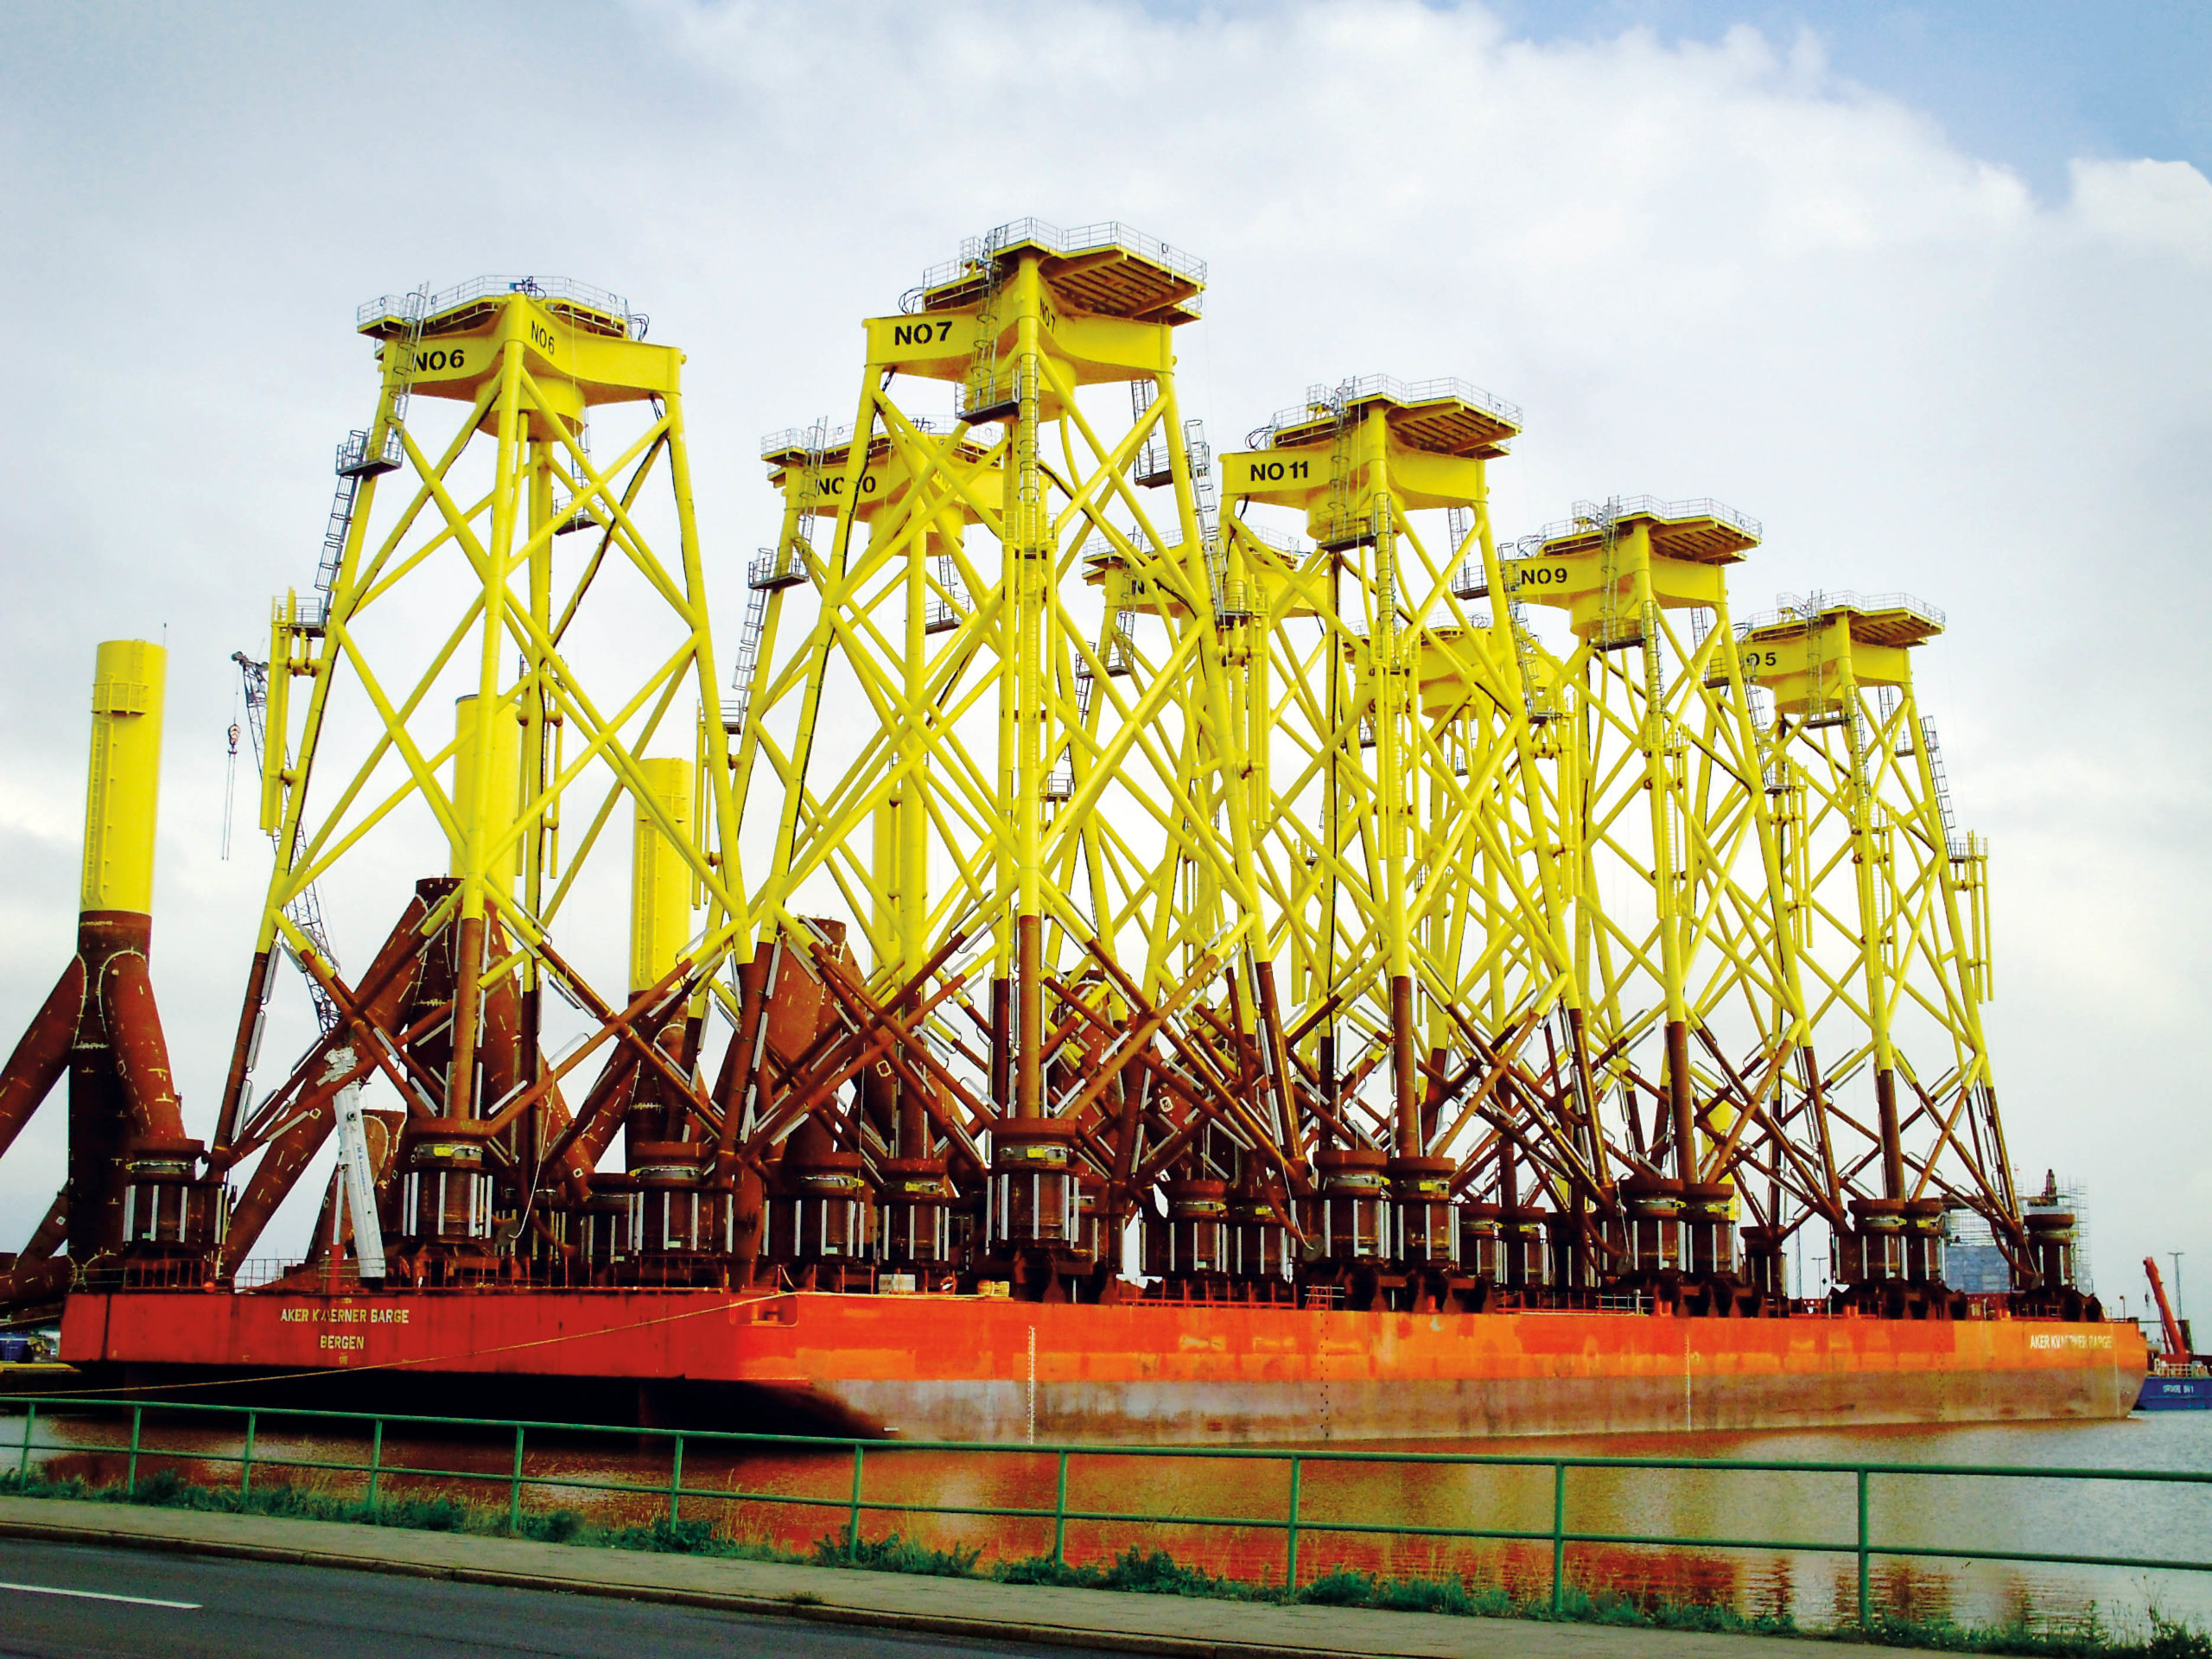
\includegraphics[height=0.7\textheight,trim={12cm 15cm 40cm 0},clip]{images/jacket.jpg}
    \end{columns}
\end{frame}

\begin{frame}{Example}
    \begin{center}
        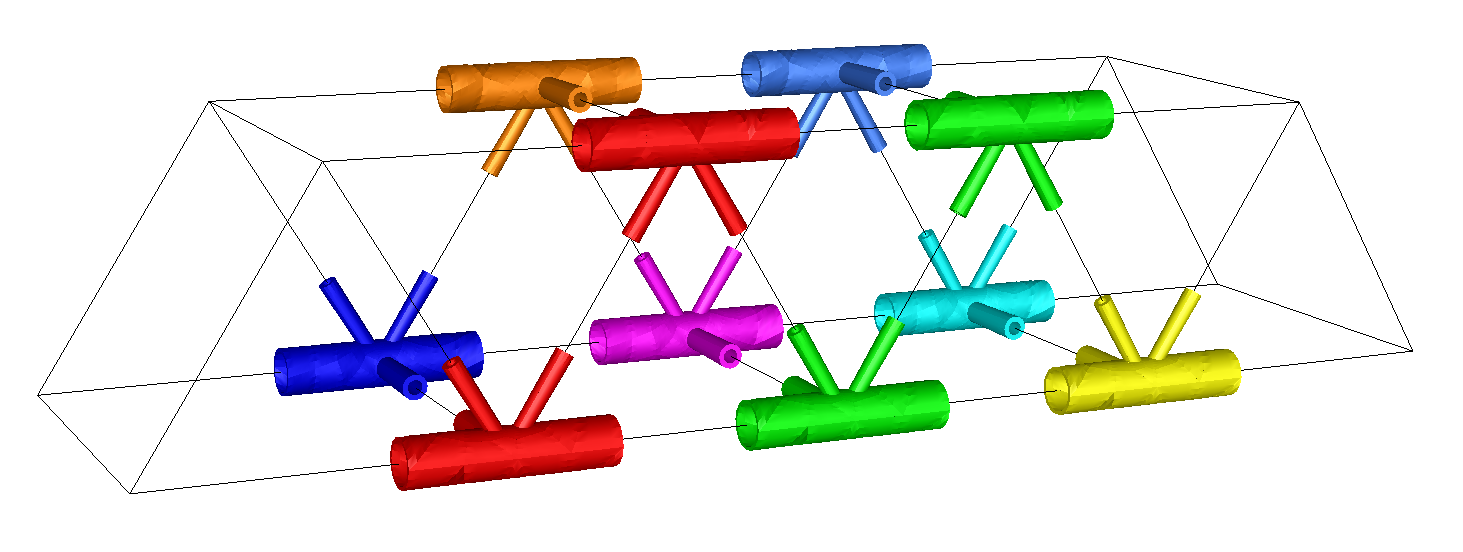
\includegraphics[width=1.0\textwidth,trim={0 0 0 0},clip]{images/ebridge-before.png}
    \end{center}
\end{frame}

\begin{frame}{Static condensation}
    \begin{columns}
        \column{0.7\linewidth}
        \begin{itemize}
            \item Static condensation `compresses' each component to a \(6n \times 6n\) superelement that acts as coupling terms between otherwise disconnected beam elements.
            \item Works well if each component is \emph{identical}.
            \item Still requires the solution of a nontrivial system.
            \item Not parametrized over geometry, material, etc.
        \end{itemize}
        \column{0.3\linewidth}
        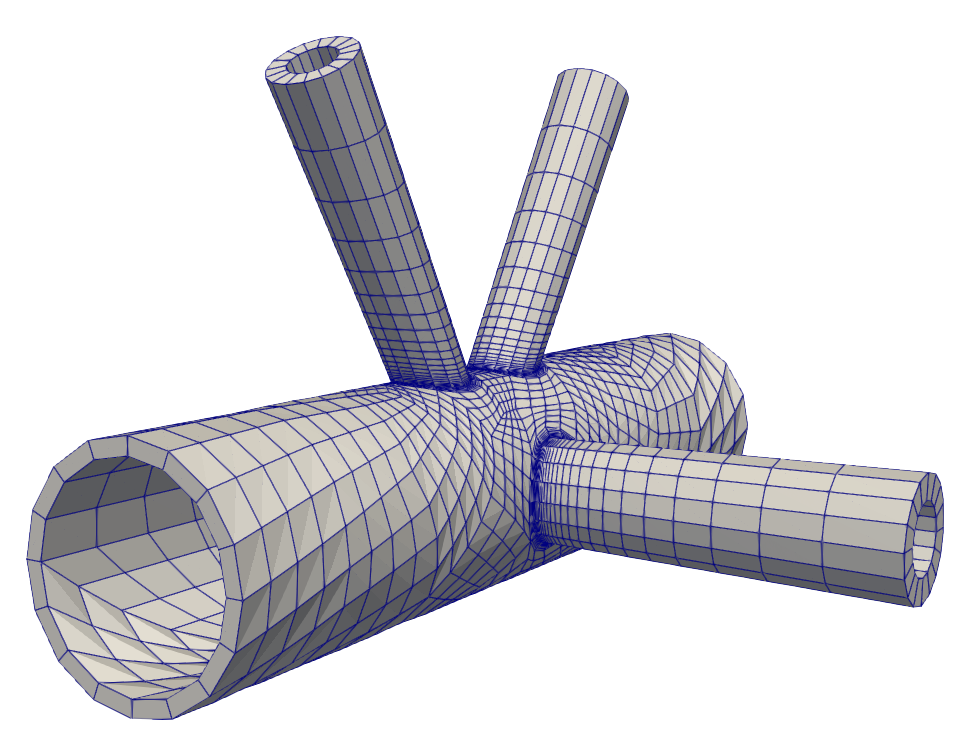
\includegraphics[height=0.4\textheight,trim={0 0 0 0},clip]{images/kjoint.png}
    \end{columns}
\end{frame}

\begin{frame}{Static condensation}
    \begin{align*}
        \begin{pmatrix}
            \mathbf A_{BB} & \mathbf A_{BI} \\
            \mathbf A_{IB} & \mathbf A_{II}
        \end{pmatrix}
        \begin{pmatrix}
            \mathbf u_B \\ \mathbf u_I
        \end{pmatrix}
        &=
        \begin{pmatrix}
            \mathbf f_B \\ \mathbf f_I
        \end{pmatrix} \\[5mm]
        \mathbf A_{II} \mathbf u_I &= \mathbf f_I - \mathbf A_{IB} \mathbf u_B \\[2mm]
        (\mathbf A_{BB} - \mathbf A_{BI} \mathbf A_{II}^{-1} \mathbf A_{IB}) \mathbf u_B
            &= \mathbf f_B - \mathbf A_{BI} \mathbf A_{II}^{-1} \mathbf f_I
    \end{align*}
\end{frame}

\begin{frame}{Port condensation}
    \begin{columns}
        \column{0.7\linewidth}
        \only<1>{The technique follows in brief Eftang and Patera (2013).}
        \begin{itemize}
            \only<1>{
                \item For each \emph{port}, six ROMs are constructed - each evaluating the response on the structure from one degree of freedom on the boundary (three translations and three rotations)
                \item In addition, one ROM is constructed with \emph{homogeneous} boundary conditions, evaluating the response from other sources, e.g.~gravity
            }
            \only<2>{
                \item In the online stage, each of the \(6n\) ROMs are queried and the solutions form the internal basis functions for a \(6n \times 6n\) superelement matrix
                \item The solution to the homogenous ROM enters the right hand side as a load term
                \item \emph{Parametrized} and \emph{faster} static condensation
            }
        \end{itemize}
        \column{0.3\linewidth}
        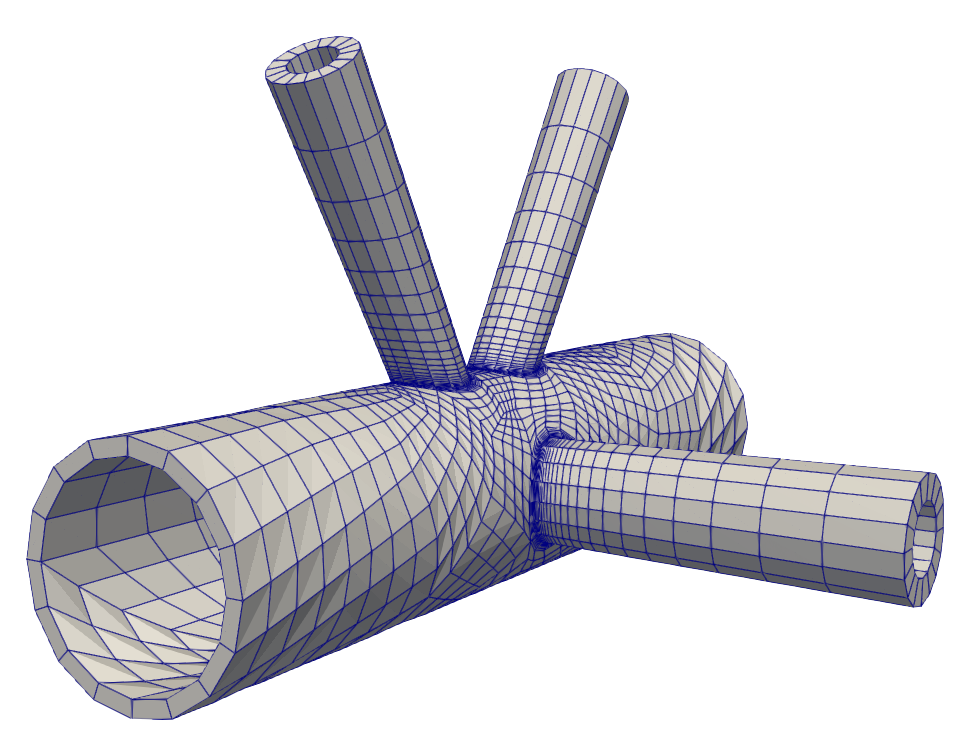
\includegraphics[height=0.4\textheight,trim={0 0 0 0},clip]{images/kjoint.png}
    \end{columns}
\end{frame}

\begin{frame}{Port condensation}
    Let
    \begin{itemize}
        \item \(\ell^{(i)}\) be the lifting function associated with port \(i\)
        \item \(\left\{b_k^{(i)}\right\}_k\) be reduced basis functions associated with port \(i\)
    \end{itemize}
    Then the response due to excitation of port \(i\) is
    \begin{align*}
        \Psi^{(i)} &= \ell^{(i)} + \sum_k c_k b_k^{(i)} \\
        a(\Psi^{(i)}, v) &= 0 \quad\forall v
    \end{align*}
\end{frame}

\begin{frame}{Port condensation}
    And the contribution to the (Galerkin) superelement is
    \begin{align*}
        a(\Psi^{(i)}, \Psi^{(j)})
        &= a\left(\Psi^{(i)}, \ell^{(j)} + \sum_l c_l b_l^{(j)} \right) \\
        &\approx a\left(\Psi^{(i)}, \ell^{(j)}\right) \\
        &= a\left(\ell^{(i)}, \ell^{(j)}\right) + \sum_k c_k a\left( b_k^{(i)}, \ell^{(j)} \right)
    \end{align*}
    where we can discard the expensive terms due to (approximate) Galerkin orthogonality.
\end{frame}

\begin{frame}{Example}
    \begin{center}
        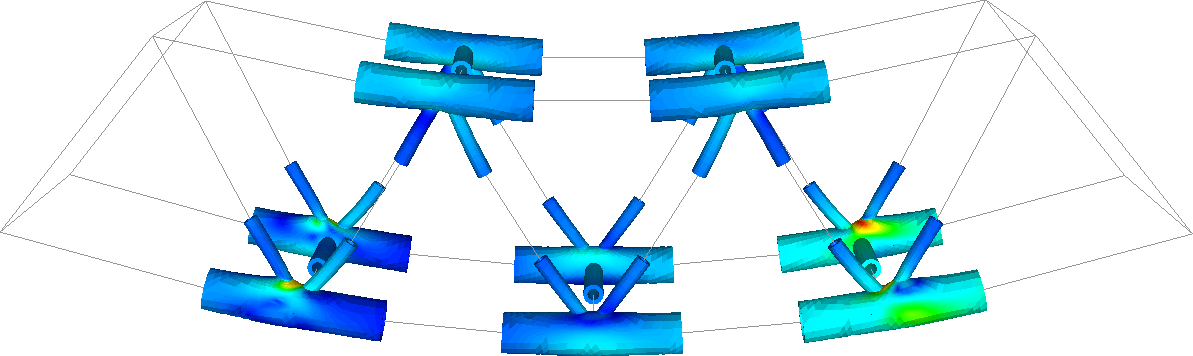
\includegraphics[width=1.0\textwidth,trim={0 0 0 0},clip]{images/ebridge-after.png}
    \end{center}
\end{frame}

\begin{frame}{Intrusiveness}
    \begin{itemize}
        \item Many decisions made in the following are motivated by non-intrusiveness
        \item RBMs are typically quite intrusive: to reduce a FOM requires expert knowledge of it
        \item We aim to deliver a generalized RBM software package (AROMA) that is as non-intrusive as possible
        \begin{itemize}
            \item snapshots as fully-featured solution vectors
            \item stiffness matrix and load vector in restricted sense (i.e.~with fixed DoFs removed and lift applied) --- avaliable as debug output in most FOM software
            \item knowledge of DoF classification (fixed/free) and lift --- fairly mundane
        \end{itemize}
        \item Aim is to view the FOM as a nearly opaque black box
    \end{itemize}
\end{frame}

\begin{frame}{Reduced basis methods}
    Substitute the solution of a large system
    \begin{center}
        \begin{tikzpicture}[scale=0.35]
            \fill[sintefyellow, draw=sintefblue, very thick, rounded corners=1mm] (0,0) rectangle (5,5);
            \fill[sinteflightgrey, draw=sintefblue, very thick, rounded corners=1mm] (5.5,0) rectangle (6.5,5);
            \fill[sinteflightgrey, draw=sintefblue, very thick, rounded corners=1mm] (8.5,0) rectangle (9.5,5);
            \node at (2.5,2.5) {$\mathbf A$};
            \node at (6.0,2.5) {$\mathbf u$};
            \node at (7.5,2.5) {$=$};
            \node at (9.0,2.5) {$\mathbf f$};
        \end{tikzpicture}
    \end{center}
    with a smaller one
    \begin{center}
        \begin{tikzpicture}[scale=0.35]
            \fill[sintefyellow, draw=sintefblue, very thick, rounded corners=1mm] (-5.5,1) rectangle (-0.5,4);
            \fill[sintefyellow, draw=sintefblue, very thick, rounded corners=1mm] (0,0) rectangle (5,5);
            \fill[sintefyellow, draw=sintefblue, very thick, rounded corners=1mm] (5.5,0) rectangle (8.5,5);
            \fill[sinteflightgrey, draw=sintefblue, very thick, rounded corners=1mm] (9,1) rectangle (10,4);
            \fill[sintefyellow, draw=sintefblue, very thick, rounded corners=1mm] (12,1) rectangle (17,4);
            \fill[sinteflightgrey, draw=sintefblue, very thick, rounded corners=1mm] (17.5,0) rectangle (18.5,5);
            \node at (-3,2.5) {$\mathbf V^\intercal$};
            \node at (2.5,2.5) {$\mathbf A$};
            \node at (7,2.5) {$\mathbf V$};
            \node at (11,2.5) {$=$};
            \node at (14.5,2.5) {$\mathbf V^\intercal$};
            \node at (18,2.5) {$\mathbf f$};
            \draw (5.5,5.8) -- (5.5, 6) -- (10,6) -- (10,5.8);
            \draw (-5.5,-0.8) -- (-5.5, -1) -- (8.5,-1) -- (8.5,-0.8);
            \draw (9,-0.8) -- (9, -1) -- (10,-1) -- (10,-0.8);
            \draw (12,-0.8) -- (12, -1) -- (18.5,-1) -- (18.5,-0.8);
            \node[anchor=north] at (1.5,-1) {$\mathbf A^\mathup{r}$};
            \node[anchor=south] at (7.75,6) {$\mathbf u$};
            \node[anchor=north] at (9.5,-1) {$\mathbf u^\mathup{r}$};
            \node[anchor=north] at (15.25,-1) {$\mathbf f^\mathup{\,r}$};
        \end{tikzpicture}
    \end{center}
\end{frame}

\begin{frame}{Solution and assembly}
    \begin{itemize}
        \item Extremely fast \emph{solutions} in the online stage: \( \mathbf A^\mathup{r}(\mu) \) frequently on the order of \( \sim 10 \times 10 \) or so.
        \item Assembly of \( \mathbf A^\mathup{r}(\mu) \) remains an open issue. On the face of it,
        \[
            \mathbf A^\mathup{r} (\mu) = \mathbf V^\intercal \mathbf A(\mu) \mathbf V
        \]
        requires the construction of the full-order matrix \( \mathbf{A}(\mu) \) in the online stage.
        \item Many solutions have been proposed, most of which relates to...
    \end{itemize}
\end{frame}

\begin{frame}{The assumption of affine parametric dependence}
    If \( \mathbf A(\mu) \) takes the form
    \[
        \mathbf A(\mu) = \sum_i \xi_i(\mu) \mathbf A_i
    \]
    then \( \mathbf A^\mathup{r}(\mu) \) takes the form
    \[
        \mathbf A^\mathup{r}(\mu) = \mathbf V^\intercal \mathbf A(\mu) \mathbf V = \sum_i \xi_i(\mu) \mathbf V^\intercal \mathbf A_i \mathbf V = \sum_i \xi_i(\mu) \mathbf A^\mathup{r}_i
    \]
    Each $\mathbf A^\mathup{r}_i$ is small and easily storeable. Assuming the $\xi_i$ are not pathological and the sum not too long, assembly in this form is competitive with time spent solving the system.
\end{frame}

\begin{frame}{The assumption of affine parametric dependence}
    \begin{itemize}
        \item Affinity tends to hold well with
        \begin{itemize}
            \item explicit material parameters: elastic properties, viscosities, thermal conductivities
            \item load and boundary data
        \end{itemize}
        \item But not with geometric variability
        \begin{itemize}
            \item even simple variation manifests in the integrands (for FEM) or fluxes (for FVM) in nontrivial ways (Fonn et.~al., 2018)
        \end{itemize}
        \item Approximate affine parametric dependence can be \emph{forced} using various interpolation methods
    \end{itemize}
\end{frame}

\begin{frame}{Empirical Interpolation}
    \begin{columns}
        \column{0.7\linewidth}
        \begin{itemize}
            \item EIM requires the online stage to evaluate a function \(g(x,\mu)\) at certain points \(x\) in the physical domain, or a vector-valued function \(g_i(\mu)\) at certain entries \(i\).
            \item Here, \(g\) is the Finite Element variational form or similar for FVM
            \item In the black-box FOM context we operate in, such restricted evaluation of the integrand is not possible (too intrusive)
            \item Instead, we resort to Matrix Least Squares
        \end{itemize}
        \column{0.3\linewidth}
        \begin{tikzpicture}[scale=3]
            \draw (0,0) rectangle (1,1);
            \draw[fill=sintefyellow] (0.45,0) rectangle (0.55,1);
            \draw[fill=sintefblue] (0.5,0.1) circle (0.03);
            \draw[fill=sintefblue] (0.5,0.2) circle (0.03);
            \draw[fill=sintefblue] (0.5,0.7) circle (0.03);
            \node[anchor=north] at (0.5,0) {\(\mu\)};
            \node[anchor=east] at (0,0.5) {\(x\)};
        \end{tikzpicture}
        % 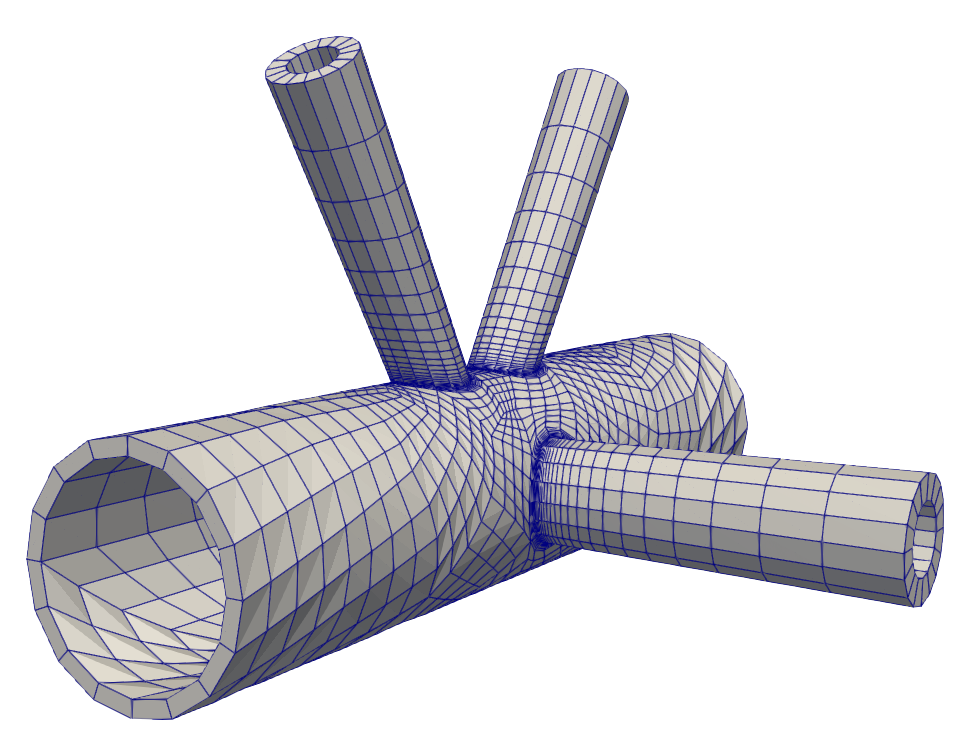
\includegraphics[height=0.4\textheight,trim={0 0 0 0},clip]{images/kjoint.png}
    \end{columns}
\end{frame}

\begin{frame}{Matrix Least Squares}
    Given reasonable guesses for \(\xi_i(\mu)\), compute corresponding coefficient matrices \(\mathbf A_i\) by minimizing
    \[
        \int_\mu \, \left\| \mathbf A(\mu) - \sum_i \xi_i(\mu) \mathbf A_i \right\|^2_2 \mathup{d}\mu.
    \]
    In practice, this is implemented the same was as conventional \(L^2\)-fit on a sampling over \(\mu\):
    \begin{align*}
        \mathbf B_{ji} &= \xi_i(\mu_j) \\
        \mathbf A_i &= \sum_{jk} (\mathbf B^\intercal \mathbf B)_{ik}^{-1} \mathbf B_{jk} \mathbf A(\mu_j)
    \end{align*}
\end{frame}

\begin{frame}{Matrix Least Squares}
    \begin{itemize}
        \item In practice, sampling \(\mathbf A, \mathbf f\) is done at the same time, and in the same parameter values as the snapshots.
        \item If the sampling strategy is known in advance, the contribution from \(\mathbf A(\mu_j)\) can be immediately applied and the matrix then discarded.
        \item Much leeway is admitted in the choice of \(\xi_i\)
        \begin{itemize}
            \item known affinities may be exploited, e.g.~
            \[
                \xi_1(E,\nu) = \frac{E}{2(1+\nu)}, \qquad \xi_2(E,\nu) = \frac{E}{(1-2\nu)(1+\nu)}
            \]
            \item orthogonal polynomial families as a last resort, \( \xi_i(r) = P_i(r) \)
            \item a combination, \( \xi_i(E,\nu) = E P_i(\nu) \)
        \end{itemize}
    \end{itemize}
\end{frame}

\begin{frame}{Example: two-port cylinder}
    \begin{columns}
        \column{0.5\linewidth}
        Minimal example with variable radius \\
        \vspace{1cm}
        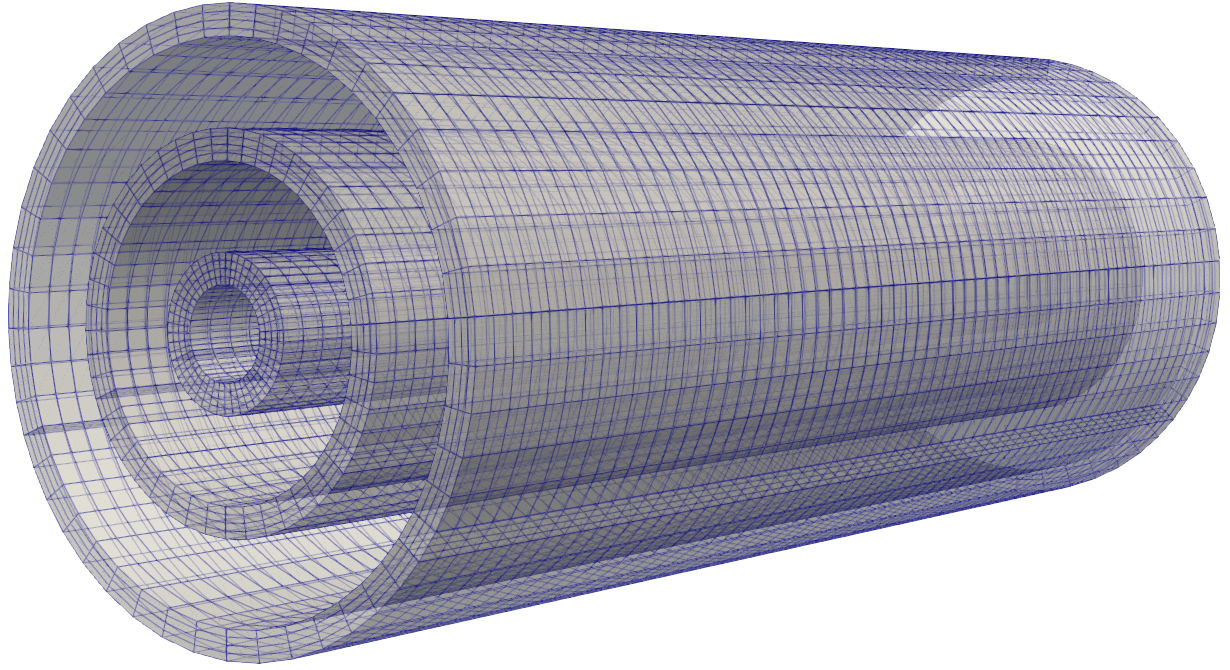
\includegraphics[height=0.4\textheight,trim={0 0 0 0},clip]{images/radii.png}
        \column{0.5\linewidth}
        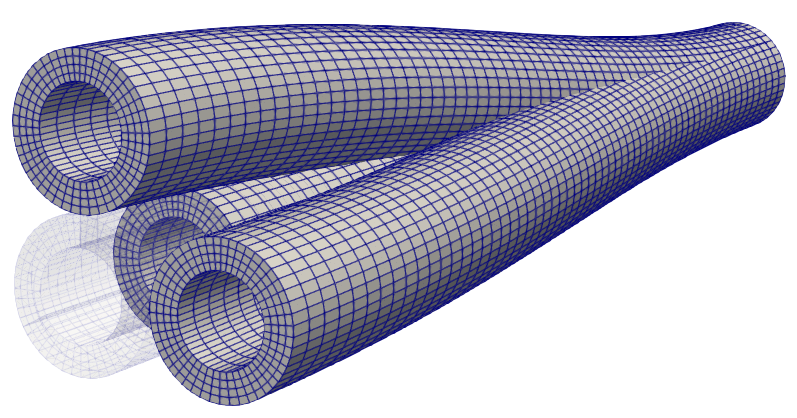
\includegraphics[height=0.4\textheight,trim={0 0 0 0},clip]{images/transdofs.png}
        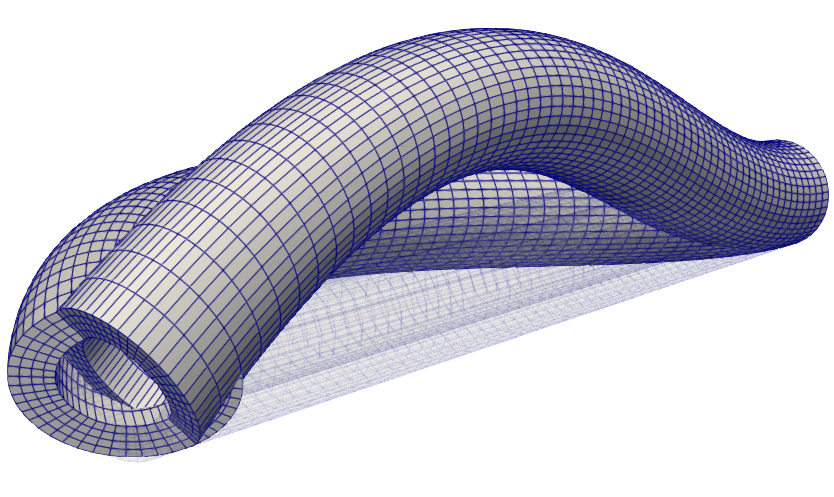
\includegraphics[height=0.45\textheight,trim={0 0 0 0},clip]{images/rotdofs.png}
    \end{columns}
\end{frame}

\begin{frame}[fragile]
    \begin{center}
        \begin{tikzpicture}
            \begin{axis}[
                ymode=log,
                xlabel={Polynomial degree},
                ylabel={Relative error},
                width=\textwidth,
                height=\textheight,
                grid=both,
            ]
                \addplot[sintefcyan, thick, mark=*] table[x index={0},    y index={1}]{data/interrs-maxrel.csv};
                \addplot[sintefmagenta, thick, mark=*] table[x index={0}, y index={2}]{data/interrs-maxrel.csv};
                \addplot[sintefblue, thick, mark=*] table[x index={0},  y index={3}]{data/interrs-maxrel.csv};
                \addplot[sintefgrey, thick, mark=*] table[x index={0},  y index={5}]{data/interrs-maxrel.csv};
                \addplot[sintefyellow, thick, mark=*] table[x index={0},  y index={6}]{data/interrs-maxrel.csv};
                \addplot[sintefcyan, thick, mark=*, dashed] table[x index={0},    y index={1}]{data/interrs-meanrel.csv};
                \addplot[sintefmagenta, thick, mark=*, dashed] table[x index={0}, y index={2}]{data/interrs-meanrel.csv};
                \addplot[sintefblue, thick, mark=*, dashed] table[x index={0},  y index={3}]{data/interrs-meanrel.csv};
                \addplot[sintefgrey, thick, mark=*, dashed] table[x index={0},  y index={5}]{data/interrs-meanrel.csv};
                \addplot[sintefyellow, thick, mark=*, dashed] table[x index={0},  y index={6}]{data/interrs-meanrel.csv};
                \legend{
                    Homogeneous,
                    Parallel translation,
                    Transverse translation,
                    Parallel rotation,
                    Transverse rotation,
                }
            \end{axis}
        \end{tikzpicture}
    \end{center}
\end{frame}

\begin{frame}[fragile]{Homogenous case}
    \vspace{-.2cm}
    \begin{center}
        \begin{tikzpicture}
            \begin{axis}[
                ymode=log,
                xlabel={Polynomial degree},
                ylabel={Relative error},
                width=\textwidth,
                height=0.9\textheight,
                grid=both,
                legend pos=south west,
            ]
                \addplot[sintefblue, thick, mark=*] table[x index={0}, y index={1}]{data/romerrs-maxrel-homogeneous.csv};
                \addplot[sintefcyan, thick, mark=*] table[x index={0}, y index={2}]{data/romerrs-maxrel-homogeneous.csv};
                \addplot[sintefmagenta, thick, mark=*] table[x index={0}, y index={3}]{data/romerrs-maxrel-homogeneous.csv};
                \addplot[sintefyellow, thick, mark=*] table[x index={0}, y index={4}]{data/romerrs-maxrel-homogeneous.csv};
                \addplot[sintefgrey, thick, mark=*] table[x index={0}, y index={8}]{data/romerrs-maxrel-homogeneous.csv};
                \addplot[sintefblue, thick, mark=*, dashed] table[x index={0}, y index={1}]{data/romerrs-meanrel-homogeneous.csv};
                \addplot[sintefcyan, thick, mark=*, dashed] table[x index={0}, y index={2}]{data/romerrs-meanrel-homogeneous.csv};
                \addplot[sintefmagenta, thick, mark=*, dashed] table[x index={0}, y index={3}]{data/romerrs-meanrel-homogeneous.csv};
                \addplot[sintefyellow, thick, mark=*, dashed] table[x index={0}, y index={4}]{data/romerrs-meanrel-homogeneous.csv};
                \addplot[sintefgrey, thick, mark=*, dashed] table[x index={0}, y index={8}]{data/romerrs-meanrel-homogeneous.csv};
                \legend{
                    \(M=1\),
                    \(M=2\),
                    \(M=3\),
                    \(M=4\),
                    \(M=8\),
                }
            \end{axis}
        \end{tikzpicture}
    \end{center}
\end{frame}

\begin{frame}[fragile]{Parallel translation case}
    \vspace{-1cm}
    \begin{center}
        \begin{tikzpicture}
            \begin{axis}[
                ymode=log,
                xlabel={Polynomial degree},
                ylabel={Relative error},
                width=\textwidth,
                height=0.9\textheight,
                grid=both,
                legend pos=south west,
            ]
                \addplot[sintefblue, thick, mark=*] table[x index={0}, y index={1}]{data/romerrs-maxrel-ptrans.csv};
                \addplot[sintefcyan, thick, mark=*] table[x index={0}, y index={2}]{data/romerrs-maxrel-ptrans.csv};
                \addplot[sintefmagenta, thick, mark=*] table[x index={0}, y index={3}]{data/romerrs-maxrel-ptrans.csv};
                \addplot[sintefyellow, thick, mark=*] table[x index={0}, y index={4}]{data/romerrs-maxrel-ptrans.csv};
                \addplot[sintefgrey, thick, mark=*] table[x index={0}, y index={8}]{data/romerrs-maxrel-ptrans.csv};
                \addplot[sintefblue, thick, mark=*, dashed] table[x index={0}, y index={1}]{data/romerrs-meanrel-ptrans.csv};
                \addplot[sintefcyan, thick, mark=*, dashed] table[x index={0}, y index={2}]{data/romerrs-meanrel-ptrans.csv};
                \addplot[sintefmagenta, thick, mark=*, dashed] table[x index={0}, y index={3}]{data/romerrs-meanrel-ptrans.csv};
                \addplot[sintefyellow, thick, mark=*, dashed] table[x index={0}, y index={4}]{data/romerrs-meanrel-ptrans.csv};
                \addplot[sintefgrey, thick, mark=*, dashed] table[x index={0}, y index={8}]{data/romerrs-meanrel-ptrans.csv};
                \legend{
                    \(M=1\),
                    \(M=2\),
                    \(M=3\),
                    \(M=4\),
                    \(M=8\),
                }
            \end{axis}
        \end{tikzpicture}
    \end{center}
\end{frame}

\begin{frame}[fragile]{Transverse translation case}
    \vspace{-.2cm}
    \begin{center}
        \begin{tikzpicture}
            \begin{axis}[
                ymode=log,
                xlabel={Polynomial degree},
                ylabel={Relative error},
                width=\textwidth,
                height=0.9\textheight,
                grid=both,
                legend pos=south west,
            ]
                \addplot[sintefblue, thick, mark=*] table[x index={0}, y index={1}]{data/romerrs-maxrel-ttrans.csv};
                \addplot[sintefcyan, thick, mark=*] table[x index={0}, y index={2}]{data/romerrs-maxrel-ttrans.csv};
                \addplot[sintefmagenta, thick, mark=*] table[x index={0}, y index={3}]{data/romerrs-maxrel-ttrans.csv};
                \addplot[sintefyellow, thick, mark=*] table[x index={0}, y index={4}]{data/romerrs-maxrel-ttrans.csv};
                \addplot[sintefgrey, thick, mark=*] table[x index={0}, y index={8}]{data/romerrs-maxrel-ttrans.csv};
                \addplot[sintefblue, thick, mark=*, dashed] table[x index={0}, y index={1}]{data/romerrs-meanrel-ttrans.csv};
                \addplot[sintefcyan, thick, mark=*, dashed] table[x index={0}, y index={2}]{data/romerrs-meanrel-ttrans.csv};
                \addplot[sintefmagenta, thick, mark=*, dashed] table[x index={0}, y index={3}]{data/romerrs-meanrel-ttrans.csv};
                \addplot[sintefyellow, thick, mark=*, dashed] table[x index={0}, y index={4}]{data/romerrs-meanrel-ttrans.csv};
                \addplot[sintefgrey, thick, mark=*, dashed] table[x index={0}, y index={8}]{data/romerrs-meanrel-ttrans.csv};
                \legend{
                    \(M=1\),
                    \(M=2\),
                    \(M=3\),
                    \(M=4\),
                    \(M=8\),
                }
            \end{axis}
        \end{tikzpicture}
    \end{center}
\end{frame}

\begin{frame}[fragile]{Parallel rotation case}
    \vspace{-1cm}
    \begin{center}
        \begin{tikzpicture}
            \begin{axis}[
                ymode=log,
                xlabel={Polynomial degree},
                ylabel={Relative error},
                width=\textwidth,
                height=0.9\textheight,
                grid=both,
                legend pos=south west,
            ]
                \addplot[sintefblue, thick, mark=*] table[x index={0}, y index={1}]{data/romerrs-maxrel-prot.csv};
                \addplot[sintefcyan, thick, mark=*] table[x index={0}, y index={2}]{data/romerrs-maxrel-prot.csv};
                \addplot[sintefmagenta, thick, mark=*] table[x index={0}, y index={3}]{data/romerrs-maxrel-prot.csv};
                \addplot[sintefyellow, thick, mark=*] table[x index={0}, y index={4}]{data/romerrs-maxrel-prot.csv};
                \addplot[sintefgrey, thick, mark=*] table[x index={0}, y index={8}]{data/romerrs-maxrel-prot.csv};
                \addplot[sintefblue, thick, mark=*, dashed] table[x index={0}, y index={1}]{data/romerrs-meanrel-prot.csv};
                \addplot[sintefcyan, thick, mark=*, dashed] table[x index={0}, y index={2}]{data/romerrs-meanrel-prot.csv};
                \addplot[sintefmagenta, thick, mark=*, dashed] table[x index={0}, y index={3}]{data/romerrs-meanrel-prot.csv};
                \addplot[sintefyellow, thick, mark=*, dashed] table[x index={0}, y index={4}]{data/romerrs-meanrel-prot.csv};
                \addplot[sintefgrey, thick, mark=*, dashed] table[x index={0}, y index={8}]{data/romerrs-meanrel-prot.csv};
                \legend{
                    \(M=1\),
                    \(M=2\),
                    \(M=3\),
                    \(M=4\),
                    \(M=8\),
                }
            \end{axis}
        \end{tikzpicture}
    \end{center}
\end{frame}

\begin{frame}[fragile]{Transverse rotation case}
    \vspace{-.2cm}
    \begin{center}
        \begin{tikzpicture}
            \begin{axis}[
                ymode=log,
                xlabel={Polynomial degree},
                ylabel={Relative error},
                width=\textwidth,
                height=0.9\textheight,
                grid=both,
                legend pos=south west,
            ]
                \addplot[sintefblue, thick, mark=*] table[x index={0}, y index={1}]{data/romerrs-maxrel-trot.csv};
                \addplot[sintefcyan, thick, mark=*] table[x index={0}, y index={2}]{data/romerrs-maxrel-trot.csv};
                \addplot[sintefmagenta, thick, mark=*] table[x index={0}, y index={3}]{data/romerrs-maxrel-trot.csv};
                \addplot[sintefyellow, thick, mark=*] table[x index={0}, y index={4}]{data/romerrs-maxrel-trot.csv};
                \addplot[sintefgrey, thick, mark=*] table[x index={0}, y index={8}]{data/romerrs-maxrel-trot.csv};
                \addplot[sintefblue, thick, mark=*, dashed] table[x index={0}, y index={1}]{data/romerrs-meanrel-trot.csv};
                \addplot[sintefcyan, thick, mark=*, dashed] table[x index={0}, y index={2}]{data/romerrs-meanrel-trot.csv};
                \addplot[sintefmagenta, thick, mark=*, dashed] table[x index={0}, y index={3}]{data/romerrs-meanrel-trot.csv};
                \addplot[sintefyellow, thick, mark=*, dashed] table[x index={0}, y index={4}]{data/romerrs-meanrel-trot.csv};
                \addplot[sintefgrey, thick, mark=*, dashed] table[x index={0}, y index={8}]{data/romerrs-meanrel-trot.csv};
                \legend{
                    \(M=1\),
                    \(M=2\),
                    \(M=3\),
                    \(M=4\),
                    \(M=8\),
                }
            \end{axis}
        \end{tikzpicture}
    \end{center}
\end{frame}

\begin{frame}{Wish list}
    \begin{itemize}
        \item Ability to both
        \begin{itemize}
            \item not plan sampling scheme in advance, \emph{and}
            \item be able use and discard matrices on-the-fly
        \end{itemize}
        \item Discover suitable $\xi$ automatically
        \item Maintain black-box treatment of FOM
        \item Some more complicated case studies (meshing challenges)
    \end{itemize}
\end{frame}

\backmatter

\end{document}
